\documentclass[twocolumn,10pt]{article}

% ---- Packages ----
\usepackage{amsmath,amssymb,amsfonts}
\usepackage{booktabs}
\usepackage{graphicx}
\usepackage{xcolor}
\usepackage{hyperref}
\usepackage[margin=0.75in]{geometry}
\usepackage{caption}
\usepackage{natbib}
\bibliographystyle{plainnat}
\usepackage{authblk}
\usepackage[T1]{fontenc}
\usepackage{microtype}
\usepackage{enumitem}
\setlist{nosep,leftmargin=*}

% ---- Metadata ----
\title{\textbf{Information-Theoretic Constraints on Immune Recognition:\\Antigenic Entropy, Signaling Bottlenecks, and the\\Host--Pathogen Learning Race}}

\author[1]{Tana Kieper\thanks{Correspondence: tana@protogenbio.com}}
\author[1]{Lennart Lopin\thanks{ORCID: 0009-0001-2751-2060. Email: lennart@protogenbio.com}}
\affil[1]{Protogen Bio Corporation}

\date{April 2026}

\begin{document}
\maketitle
\thispagestyle{empty}

% ============================================================
% ABSTRACT
% ============================================================
\begin{abstract}
Immune signaling channels have measured information-processing capacities: the TNF$\to$NF-$\kappa$B pathway transmits $0.92 \pm 0.01$~bits per cell per interaction~\citep{cheong2011}, and even multi-feature dynamic encoding reaches only ${\sim}2.6$~bits~\citep{adelaja2021}.  We ask whether antigenic diversity in three canonical immune-evasion systems exceeds these per-interaction capacities.  For \textit{Trypanosoma brucei}, VSG expression entropy oscillates between 0.04 and 3.99~bits over the course of murine infection~\citep{mugnier2015}, crossing above and below the ${\sim}1$-bit capacity threshold as the host clears dominant variants and the parasite switches---a temporal pattern consistent with a capacity-limited recognition channel.  We estimate the rate of antigenic novelty generation at ${\sim}0.04\text{--}0.06$~bits/day, approximately matched by the immune learning rate of ${\sim}0.07\text{--}0.14$~bits/day, consistent with the observed chronic-but-survivable infection dynamics.  For \textit{Plasmodium falciparum}, global var gene entropy is $6.79$~bits [95\% CI: 6.76, 6.79] across 2,398 isolates~\citep{otto2019}---though only one var gene is expressed at a time, so this measures the sequential switching repertoire available across chronic infection, not simultaneous antigenic load.  For HIV-1, mean per-position envelope entropy is 2.98~bits [2.94, 3.03] across 496 sequences, the most extreme $H/C$ ratio but also the weakest biological match to our channel model due to cross-subtype inflation.  All three systems produce antigenic source entropy exceeding per-interaction signaling capacity.  However, the immune system is not a single signaling wire: it is a distributed adaptive inference network with memory, cross-reactivity, and massive parallelism.  We use the discrete memoryless channel (DMC) because it connects to existing measurements, but our entropy estimates are upper bounds on the effective immunological challenge, and the true aggregate capacity of the immune system almost certainly exceeds our bottleneck benchmarks.  The strongest evidence for information-theoretic constraints operating \textit{in vivo} comes from the \textit{T.~brucei} oscillation dynamics.  The decisive next steps are to measure signaling capacity during active infection and to compute mutual information from paired antigen--response data.
\end{abstract}

\smallskip
\noindent\textbf{Keywords:} information theory, Shannon entropy, channel capacity, immune evasion, antigenic variation, \textit{Trypanosoma brucei}, signaling bottleneck

% ============================================================
% 1. INTRODUCTION
% ============================================================
\section{Introduction}
\label{sec:intro}

Individual immune cells make decisions with limited information.  A T~cell encountering a peptide-MHC complex must determine whether the presented antigen warrants activation or tolerance.  This decision passes through intracellular signaling cascades whose information-processing capacity has been measured: the TNF$\to$NF-$\kappa$B pathway transmits $0.92 \pm 0.01$~bits per cell at a single timepoint~\citep{cheong2011}, dynamic temporal encoding raises this to ${\sim}1.5$~bits~\citep{selimkhanov2014}, and six distinct NF-$\kappa$B ``signaling codons'' achieve ${\sim}2.6$~bits~\citep{adelaja2021}.  At the T-cell receptor itself, discrimination capacity increases across the kinetic proofreading cascade from ${\sim}0.07$~bits after initial Lck recruitment to ${\sim}1$~bit after full LAT phosphorylation~\citep{ganti2020}.

These are narrow bottlenecks.  At ${\sim}1$~bit per signaling event, a single immune cell can barely distinguish ``threat'' from ``no threat,'' let alone discriminate among dozens or hundreds of antigenically distinct pathogen variants.

Parasites that employ antigenic variation---stochastic switching among large repertoires of surface proteins---generate diversity that may exceed these per-interaction bottlenecks.  The molecular mechanisms are well characterized: \textit{Plasmodium falciparum} encodes ${\sim}60$ var genes per genome with thousands of variants across populations~\citep{otto2019}, \textit{Trypanosoma brucei} maintains ${\sim}2{,}500$ VSG genes~\citep{mugnier2015}, and HIV-1 generates continuous antigenic novelty through rapid mutation~\citep{haynes2012}.  But the connection between this diversity and the information-processing limits of the immune system has not been made quantitative.

We compute the Shannon entropy of antigenic repertoires in these three systems and compare each against published immune signaling capacity measurements.  The question is simple: does the antigenic source entropy exceed the per-interaction capacity of the signaling channels through which immune cells must process pathogen information?

We find that it does, consistently, across all three systems.  The strongest evidence comes from \textit{T.~brucei}, where VSG expression entropy oscillates above and below the ${\sim}1$-bit capacity threshold in a pattern consistent with a capacity-limited recognition process.  \textit{P.~falciparum} and HIV-1 provide supporting cases with important biological caveats that we address explicitly.

Two qualifications frame the entire paper.  First, comparing antigenic entropy to single-pathway capacity is comparing a source rate to a bottleneck, not to the full system.  The immune system is a distributed adaptive network with memory, cross-reactivity, and massive parallelism; its aggregate capacity almost certainly exceeds any single-pathway measurement.  Second, our entropy estimates are upper bounds on the effective immunological challenge, because not all sequence diversity is immunologically relevant and not all variants are encountered simultaneously.  We use the discrete memoryless channel (DMC) model because it connects directly to existing measurements, and we are explicit about where it breaks down.

\subsection{Structure of the Paper}

Section~\ref{sec:related} reviews the relevant literatures.  Section~\ref{sec:framework} presents the formal framework, including the DMC model and its limitations (Section~\ref{sec:dmc}).  Section~\ref{sec:data} describes data and methods.  Section~\ref{sec:results} presents results from three parasite systems, with the rate comparison (antigenic novelty vs.\ immune learning) integrated into the \textit{T.~brucei} analysis.  Section~\ref{sec:discussion} discusses why the naive model works as well as it does, proposes better models for future work, and addresses limitations.

% ============================================================
% 2. RELATED WORK
% ============================================================
\section{Related Work}
\label{sec:related}

\subsection{The Immune System as an Information Channel}

The application of Shannon's information theory to cellular signaling has produced a decade of rigorous measurements.  \citet{cheong2011} computed the channel capacity of the TNF$\to$NF-$\kappa$B pathway at $0.92 \pm 0.01$~bits per cell---barely sufficient for binary discrimination between ``TNF present'' and ``TNF absent.''  \citet{selimkhanov2014} showed that dynamic encoding through temporal patterns raises capacity to ${\sim}1.5$~bits.  \citet{uda2013} measured ${\sim}1$~bit for growth factor signaling through ERK, Akt, and S6 pathways.  \citet{adelaja2021} identified six distinct NF-$\kappa$B ``signaling codons'' (speed, peak, duration, total, early-vs-late, oscillation) achieving ${\sim}2.6$~bits.  Most recently, \citet{nalecz2023} demonstrated that pulsatile temporal encoding through the MAPK/ERK pathway achieves $\geq 6$~bits/hour.

For immune recognition specifically, \citet{ganti2020} showed that TCR discrimination capacity increases across the kinetic proofreading cascade: ${\sim}0.07$~bits after initial Lck recruitment, increasing to ${\sim}1$~bit after full LAT phosphorylation.  The realized TCR repertoire diversity in young adults comprises approximately $10^8$ unique TCR$\beta$ sequences (${\sim}26.6$~bits of combinatorial diversity), but the per-interaction channel capacity---how much a single TCR engagement tells the cell about antigen identity---remains near 1~bit.

\subsection{Parasitic Immune Evasion}

The molecular mechanisms of parasitic immune evasion are extensively documented but have never been quantified information-theoretically.

\textit{Plasmodium falciparum} encodes ${\sim}60$ var genes per genome, each encoding a distinct PfEMP1 surface protein.  Only one is expressed at a time, with stochastic switching at rates of ${\sim}2\%$ per generation~\citep{horrocks2004}.  Population-level surveys identify thousands of distinct variants with minimal overlap between geographic populations~\citep{barry2007,day2017,otto2019}.

\textit{Trypanosoma brucei} maintains ${\sim}2{,}500$ VSG genes per genome, with ${\sim}20\%$ potentially functional.  \citet{mugnier2015} used VSG-seq to track in vivo switching dynamics, finding that up to 100 VSGs are expressed simultaneously and that the repertoire is explored sequentially over months-long infections.

HIV-1 mutates at $3.4 \times 10^{-5}$ per nucleotide per replication cycle, generating continuous antigenic novelty.  The envelope glycoprotein (env/gp160) is the primary target of neutralizing antibodies and the most variable protein in the HIV genome.

\subsection{Information Theory in Host--Pathogen Interactions}

\citet{bellamy2024} model immune-pathogen coevolution using entropy production and information exchange rates, introducing ``co-evolutionary efficiency.''  \citet{mora2023} argue that a quantitative theory of viral-immune coevolution is within reach.  \citet{bergstrom2005} proved that the fitness value of environmental information equals the mutual information between cue and environment.  \citet{rahman2011} catalog pathogen subversion of NF-$\kappa$B---the very pathway whose channel capacity has been measured---but do not quantify the capacity reduction.  These works approach the intersection of information theory and immunology but do not measure antigenic entropy against immune channel capacity.  The synthesis we present---computing parasitic source entropy and comparing it to measured channel capacity---has not been performed.

% ============================================================
% 3. FORMAL FRAMEWORK
% ============================================================
\section{Formal Framework}
\label{sec:framework}

\subsection{The Immune Recognition Channel}

We model immune recognition as a discrete channel in Shannon's framework.  Define:
\begin{itemize}
\item \textbf{Source $X$:} The antigenic identity of an encountered entity, drawn from an antigenic alphabet $\mathcal{X}$.  For \textit{P.~falciparum}, $\mathcal{X}$ is the set of PfEMP1 domain architectures.  For \textit{T.~brucei}, $\mathcal{X}$ is the set of expressed VSG variants.  For HIV, $\mathcal{X}$ is the set of env protein sequences.
\item \textbf{Channel $P(Y|X)$:} The immune signaling cascade that transduces antigen recognition into effector output.  Characterized by the conditional distribution of immune response $Y$ given antigen $X$.
\item \textbf{Output $Y$:} The effector response---cytokine production, T-cell activation, antibody secretion, or the binary decision: attack or tolerate.
\item \textbf{Channel capacity:}
\begin{equation}
C = \max_{P(X)} I(X;Y) = \max_{P(X)} \sum_{x,y} P(x,y) \log_2 \frac{P(x,y)}{P(x)P(y)}
\label{eq:capacity}
\end{equation}
\end{itemize}

\subsection{Shannon Entropy of Antigenic Repertoires}

The Shannon entropy of the antigenic source distribution is:
\begin{equation}
H(X) = -\sum_{x \in \mathcal{X}} P(x) \log_2 P(x)
\label{eq:entropy}
\end{equation}
This measures the information content (in bits) of the antigenic signal the immune system must decode.  For a repertoire of $K$ equally likely types, $H(X) = \log_2 K$.  For non-uniform distributions, $H(X) < \log_2 K$.

\subsection{The Capacity Constraint}

Shannon's noisy channel coding theorem~\citep{shannon1948} establishes that reliable communication is possible if and only if the transmission rate $R$ satisfies $R \leq C$.  When $R > C$, the probability of decoding error is bounded away from zero---no encoding strategy can achieve reliable discrimination.

In the immune context: if the antigenic entropy $H(X)$ at a signaling bottleneck exceeds the capacity $C$ of that bottleneck, then a single signaling event cannot reliably discriminate among all antigenic variants.  The immune system can still discriminate among a subset of ${\sim}2^C$ variants per channel use, and sequential learning (affinity maturation, memory cells) allows the effective capacity to accumulate over multiple encounters.  But at any given interaction, the number of simultaneously discriminable variants is bounded by $2^C$, and if the parasite presents more diversity than this at the point of recognition, some variants will be misclassified.

\subsection{The DMC Approximation and Its Limits}
\label{sec:dmc}

The discrete memoryless channel (DMC) is the simplest model connecting our antigenic entropy measurements to published capacity benchmarks.  We use it because the capacity measurements of \citet{cheong2011}, \citet{selimkhanov2014}, and \citet{adelaja2021} were computed under DMC-like assumptions: cells are stimulated, responses are measured, and mutual information is estimated from the resulting input-output distribution.

However, the immune system is not a DMC.  It is a distributed adaptive inference system with at least four properties that the DMC ignores:

\begin{enumerate}
\item \textbf{Memory.}  Adaptive immunity stores information about previously encountered antigens in memory B and T cells.  A returning pathogen variant faces a pre-primed response, effectively expanding the channel's capacity for that variant to near-instantaneous recognition.

\item \textbf{Cross-reactivity.}  A single antibody or TCR recognizes a neighborhood of related antigens, not a single point in antigenic space.  This means the effective antigenic alphabet is smaller than sequence diversity suggests---structurally similar variants may be immunologically equivalent.

\item \textbf{Partial observability.}  The immune system does not observe the full antigenic state of an infection.  It samples antigens stochastically through dendritic cell presentation, MHC loading, and lymph node trafficking.  The relevant channel is not ``antigen $\to$ response'' but ``sampled antigen $\to$ response,'' with an additional information loss at the sampling stage.

\item \textbf{Asymmetric error costs.}  Missing a pathogen (false negative) and attacking self (false positive) have very different fitness consequences.  The immune system operates under Neyman-Pearson-like constraints~\citep{cover2006}, not the symmetric error criterion implicit in Shannon capacity.
\end{enumerate}

Despite these limitations, the DMC model is not arbitrary.  The capacity measurements we use as benchmarks were themselves made under DMC assumptions---they capture the information throughput of real signaling cascades under controlled conditions.  Our entropy estimates, computed from sequence frequency distributions, are upper bounds on the effective antigenic challenge: cross-reactivity reduces the effective alphabet, and single-variant expression (in \textit{P.~falciparum} and \textit{T.~brucei}) reduces the instantaneous presentation rate below the full repertoire entropy.  The comparison of an upper-bound source entropy to a bottleneck capacity therefore provides a conservative test: if even the upper bound falls below the bottleneck, the system is comfortably within capacity.  The fact that the upper bound consistently exceeds the bottleneck is informative, even if the precise ratio overstates the actual constraint.

% ============================================================
% 4. DATA AND METHODS
% ============================================================
\section{Data and Methods}
\label{sec:data}

\subsection{Data Sources}

We analyze three independent datasets spanning three parasite species, three laboratories, and three data types:

\textbf{Dataset~1: \textit{T.~brucei} VSG expression dynamics} (primary).  \citet{mugnier2015} performed VSG-seq on 4 mice infected with \textit{T.~brucei} EATRO~1125, sampled at 8 timepoints each (days 6--30), plus late-infection data (days 96--105).  VSG expression frequencies (percentage of trypanosome population) from supplementary databases S1--S5.  Reference genome: 3,570 VSG sequences in EATRO1125 VSGdb.  This is our primary empirical contribution because it provides temporal dynamics that directly test whether entropy oscillates around a capacity boundary.

\textbf{Dataset~2: \textit{P.~falciparum} var gene repertoires} (secondary).  \citet{otto2019} assembled near-complete var gene repertoires from 2,398 clinical isolates across 18 countries, containing 168,738 var genes with domain architecture annotations.  Data obtained from varDB (Zenodo: doi:10.5281/zenodo.3549732).  Important biological caveat: only one var gene is expressed at a time per parasite, so population-level entropy measures the sequential switching repertoire available over chronic infection, not simultaneous antigenic load.

\textbf{Dataset~3: HIV-1 envelope protein sequences} (tertiary).  500 HIV-1 env protein sequences obtained from NCBI Protein Database (Entrez: txid11676[Organism] AND env[Gene Name]).  Filtered to 496 sequences within 10\% of median length (807 analyzable positions).  Cross-subtype dataset; 80.1\% mean pairwise divergence.  This is the most extreme case but the weakest biological match to our channel model, because cross-subtype diversity inflates entropy beyond what any individual host encounters.

\subsection{Channel Capacity Benchmarks}

We compare antigenic entropy against published immune signaling channel capacity measurements (Table~\ref{tab:benchmarks}):

\begin{table}[t]
\centering
\caption{Published immune signaling channel capacity measurements.  We use $C = 0.92$~bits as the primary benchmark (most conservative, most rigorously measured).}
\label{tab:benchmarks}
\footnotesize
\begin{tabular}{@{}lclc@{}}
\toprule
Pathway & $C$ (bits) & Method & Ref. \\
\midrule
TNF$\to$NF-$\kappa$B (snap.) & $0.92 \pm 0.01$ & Binned MI & \footnotesize{\citeyear{cheong2011}} \\
TNF$\to$NF-$\kappa$B (dyn.) & ${\sim}1.5$ & Dynamic MI & \footnotesize{\citeyear{selimkhanov2014}} \\
NF-$\kappa$B codons & ${\sim}2.6$ & 6 codons & \footnotesize{\citeyear{adelaja2021}} \\
TCR proofreading & ${\sim}1.0$ & Model & \footnotesize{\citeyear{ganti2020}} \\
ERK pathway & ${\sim}1.0$ & Amplitude MI & \footnotesize{\citeyear{uda2013}} \\
MAPK/ERK (pulsatile) & ${\geq}6$/hr & Dynamic MI & \footnotesize{\citeyear{nalecz2023}} \\
\bottomrule
\end{tabular}
\end{table}

\subsection{Estimation Procedure}

For each dataset:
\begin{enumerate}
\item Define the antigenic alphabet $\mathcal{X}$ (VSG variant identities, var domain architectures, or amino acid types at each position).
\item Compute the empirical frequency distribution $\hat{P}(x) = n_x / N$.
\item Compute Shannon entropy $H(X) = -\sum_x \hat{P}(x) \log_2 \hat{P}(x)$ using \texttt{scipy.stats.entropy}.
\item Apply Miller-Madow finite-sample bias correction~\citep{miller1955}: $H_{\text{corrected}} = H_{\text{raw}} + (K-1)/(2N\ln 2)$, where $K = |\mathcal{X}|$ and $N$ is the number of observations.
\item Compute 95\% bootstrap confidence intervals from 1,000 resamples with replacement.
\end{enumerate}

\subsection{Sensitivity Analysis}

For \textit{T.~brucei}, entropy is computed per-mouse and per-timepoint, with biological replication across 4 mice.  For \textit{P.~falciparum}, entropy is computed at three taxonomic resolutions: first domain only (18 types, coarsest), full domain architecture (3,249 types), and normalized subdomains (16,089 types, finest).  For HIV, both full and deduplicated sequence sets are analyzed, and $k$-mer entropy is computed at $k = 5, 7, 9, 11, 13$ to test scaling.

% ============================================================
% 5. RESULTS
% ============================================================
\section{Results}
\label{sec:results}

\subsection{\textit{T.~brucei}: Entropy Oscillation at the Capacity Boundary}
\label{sec:tbrucei}

The mean VSG expression entropy across all 4 mice and 32 mouse-timepoints is:
\begin{equation}
H(X_{\text{VSG}}) = 1.70 \text{~bits} \quad [95\%~\text{CI}: 1.34, 2.07]
\end{equation}
with a maximum single-timepoint entropy of 3.99~bits (Mouse~1, day~26).

The most striking finding is the \emph{temporal trajectory} of entropy.  Rather than increasing monotonically (as would be expected if the parasite simply accumulated diversity), VSG entropy oscillates:
\begin{itemize}
\item \textbf{Days 6--7:} $H \approx 0.04\text{--}0.36$~bits.  A single VSG dominates at 94--99\% of the population.  Entropy is below the 0.92-bit channel capacity.  The immune system can discriminate: it ``sees'' the dominant variant.
\item \textbf{Days 12--18:} $H \approx 1.5\text{--}3.6$~bits.  Multiple VSGs are co-dominant.  Entropy exceeds channel capacity.  The immune system cannot reliably discriminate among variants at the per-interaction level.
\item \textbf{Day 24:} $H$ drops to ${\approx}0.05\text{--}2.0$~bits.  The immune system has cleared the previously dominant variant; a new dominant emerges.  Entropy briefly drops below capacity again.
\item \textbf{Days 26--30:} $H \approx 0.9\text{--}4.0$~bits.  The cycle repeats.
\end{itemize}

This oscillation pattern is consistent with a capacity-limited recognition process.  When entropy is below $C$, the immune system can identify and clear the dominant variant.  When entropy exceeds $C$, the immune system cannot reliably distinguish among co-dominant variants at the per-cell level, and the parasite population gains time to establish new dominants.

\begin{figure*}[t]
\centering
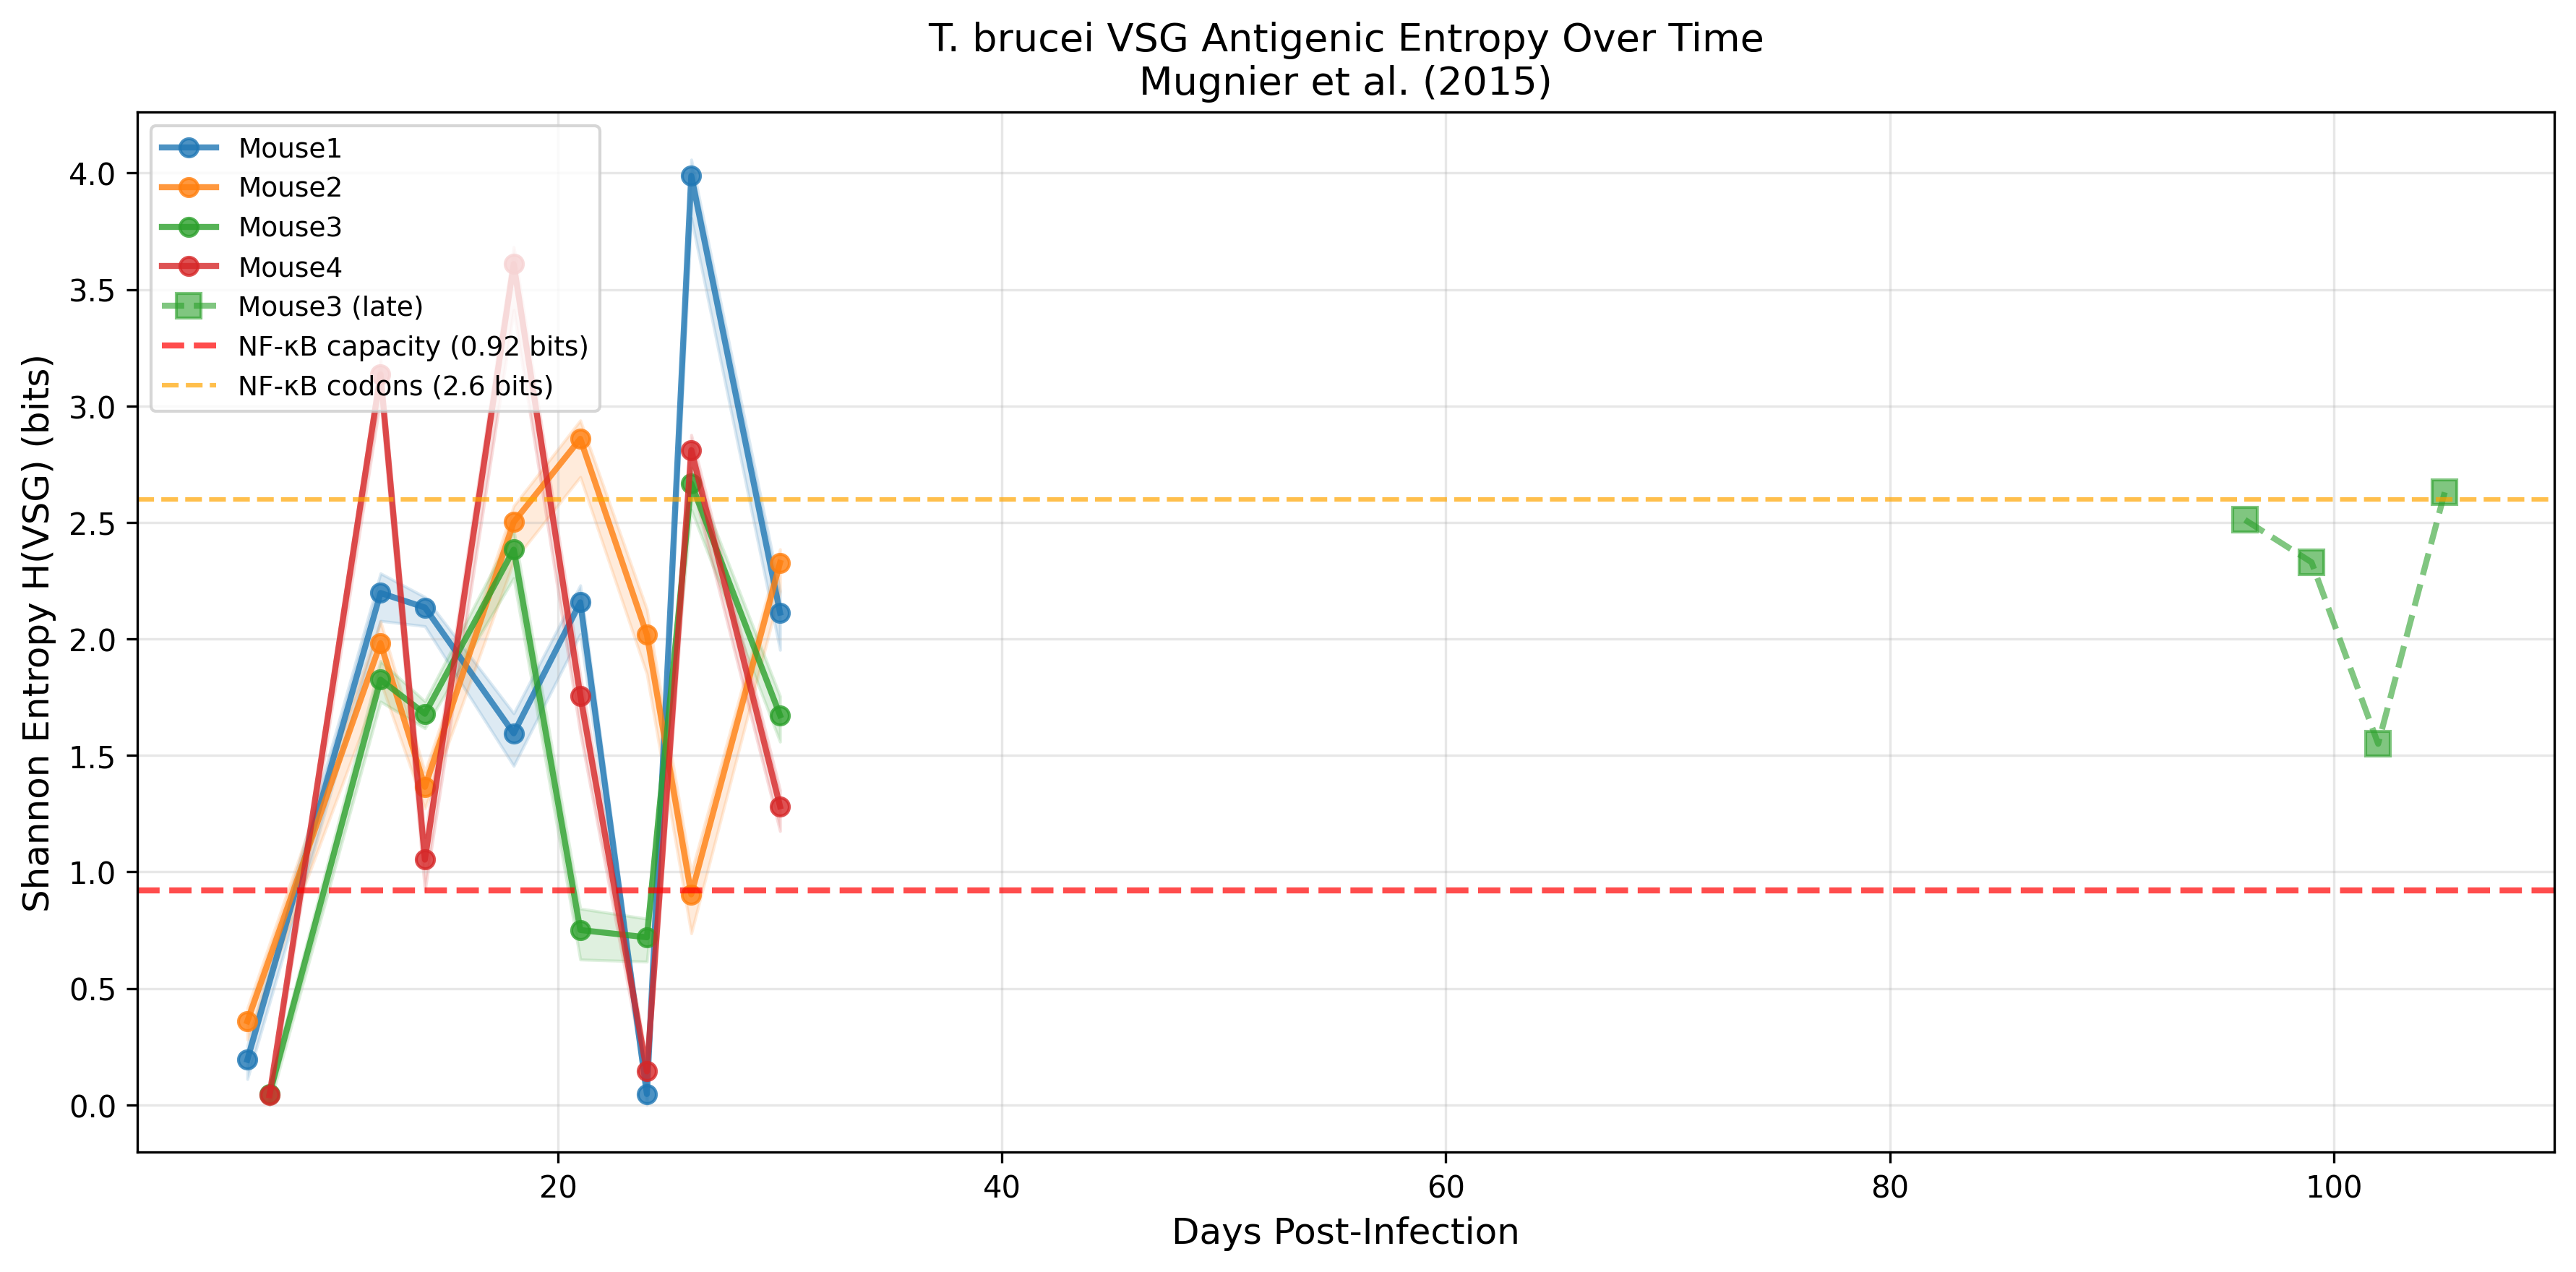
\includegraphics[width=\textwidth]{figures/fig4_tbrucei_entropy_over_time.png}
\caption{VSG expression entropy oscillates above and below the immune channel capacity threshold during \textit{T.~brucei} infection.  Four mice (EATRO~1125 strain) tracked over days 6--30.  Horizontal dashed line: NF-$\kappa$B snapshot capacity ($C = 0.92$~bits, \citealt{cheong2011}).  Entropy crosses the capacity boundary repeatedly as the immune system clears dominant variants and the parasite switches.  Shaded bands: 95\% bootstrap CIs.  Mouse~3 late-infection data (days 96--105) shown at right.}
\label{fig:tbrucei}
\end{figure*}

\textbf{Biological replication.}  Results are consistent across all 4 mice: Mouse~1 mean $H = 1.80$ [1.00, 2.59]; Mouse~2: 1.79 [1.24, 2.29]; Mouse~3: 1.47 [0.88, 2.07]; Mouse~4: 1.73 [0.85, 2.61].

\textbf{Late infection.}  At days 96--105, entropy is 2.25~bits with 97 distinct VSGs detected---confirming that the parasite maintains above-capacity diversity throughout chronic infection.

\textbf{Sequential switching structure.}  The mutual information between timepoint and VSG identity is $I(\text{time}; \text{VSG}) = 2.2\text{--}2.6$~bits across mice (87\% of temporal uncertainty resolved).  This confirms that VSG switching is sequential, not random---the parasite deploys its antigenic repertoire in a structured order.

We emphasize that the oscillation pattern was not predicted by our framework \emph{a priori}---we expected monotonic entropy increase.  The oscillation is more informative than monotonic growth: it shows that the capacity boundary, if it is indeed operating, functions as a dynamic threshold around which infection dynamics evolve.  However, the oscillation could also reflect parasitemia waves driven by resource competition or density-dependent switching rather than information-theoretic constraints.  Distinguishing these explanations requires measuring immune channel capacity directly during infection.

\subsubsection{Rate of Antigenic Novelty vs.\ Rate of Immune Learning}
\label{sec:rates}

Shannon entropy of the antigenic repertoire measures \emph{source complexity} (a stock), not the rate at which new antigens are presented (a flow).  The proper dynamic comparison is between two rates:
\begin{equation}
R_{\text{novelty}} = \frac{dH(X)}{dt} \quad \text{vs.} \quad R_{\text{learning}} = \frac{dC_{\text{effective}}}{dt}
\label{eq:rates}
\end{equation}

Our \textit{T.~brucei} data provides the most direct measurement of $R_{\text{novelty}}$.  From the entropy trajectories across 4 mice, the observed entropy growth rate is ${\sim}0.04\text{--}0.06$~bits/day (linear fit to the upward-trending envelope of the oscillating trajectory).

Against this, the immune system's learning rate can be estimated from the kinetics of adaptive immunity.  A primary antibody response to a novel antigen requires ${\sim}7\text{--}14$ days~\citep{janeway2001}; affinity maturation requires ${\sim}2\text{--}3$ weeks; memory B-cell generation requires ${\sim}4\text{--}6$ weeks.  Each ``learning event'' adds ${\sim}1$ discriminable category to the immune codebook (i.e., ${\sim}1$~bit of capacity expansion).  This gives:
\begin{equation}
R_{\text{learning}} \approx 0.07\text{--}0.14 \text{~bits/day}
\end{equation}
for the primary response.

The rates are approximately matched ($R_{\text{novelty}} \lesssim R_{\text{learning}}$), consistent with the oscillation pattern: the parasite generates antigenic novelty at a rate slightly below or comparable to immune learning, maintaining entropy above the per-interaction capacity threshold for most of the infection while the immune system periodically catches up during clearance events.  This rate-matching---rather than rate-domination in either direction---explains why trypanosome infections are chronic but not immediately lethal.  The parasite stays roughly one step ahead at the per-interaction level, even as the immune system accumulates memory that accelerates re-recognition of previously encountered variants.

\subsection{\textit{P.~falciparum}: Sequential Repertoire Entropy}
\label{sec:pfalciparum}

The global Shannon entropy over 3,249 unique var gene domain architectures across 2,398 isolates is:
\begin{equation}
H(X_{\text{global}}) = 6.79 \text{~bits} \quad [95\%~\text{CI}: 6.76, 6.79]
\end{equation}
This is $7.4\times$ the NF-$\kappa$B channel capacity ($C = 0.92$~bits) and $2.6\times$ the NF-$\kappa$B signaling codon capacity ($C = 2.6$~bits).

The mean per-isolate entropy (within individual genomes) is:
\begin{equation}
H(X_{\text{genome}}) = 4.49 \text{~bits} \quad [4.47, 4.52]
\end{equation}

Per-country entropy is remarkably consistent: 6.36--6.70~bits across the top~5 countries by sample size (Ghana, Cambodia, Malawi, Tanzania, Laos), with a cross-country mean of 6.08~bits.

\textbf{Biological caveat.}  \textit{P.~falciparum} expresses only one var gene at a time, switching stochastically at ${\sim}2\%$ per generation~\citep{horrocks2004}.  The global entropy of 6.79~bits and the per-genome entropy of 4.49~bits therefore measure the \emph{sequential switching repertoire}---the total diversity available to the parasite over the course of a chronic infection---not the simultaneous antigenic load at any given moment.  At any instant, the parasite presents a single PfEMP1 variant; the immune challenge is that the identity of that variant is drawn from a high-entropy distribution that changes over time.

This distinction matters.  The per-encounter entropy---the uncertainty the immune system faces when it encounters one infected erythrocyte---is not 4.49~bits but closer to $H_{\text{per-encounter}} = 0$ bits for a clonal population expressing a single variant, rising toward $\log_2 k$ as $k$ variants co-circulate during mixed infections.  The 4.49-bit per-genome entropy is best interpreted as an upper bound on the cumulative antigenic burden over the ${\sim}6\text{--}12$ month duration of an untreated infection, during which the parasite sequentially presents variants from its repertoire.

\textbf{Sensitivity to resolution.}  At the coarsest resolution (18 first-domain types), $H = 2.04$~bits---still $2.2\times$ the NF-$\kappa$B capacity.  At the finest resolution (16,089 normalized subdomain types), $H = 12.32$~bits.  The $H > C$ relationship holds at all resolutions.

\begin{figure}[t]
\centering
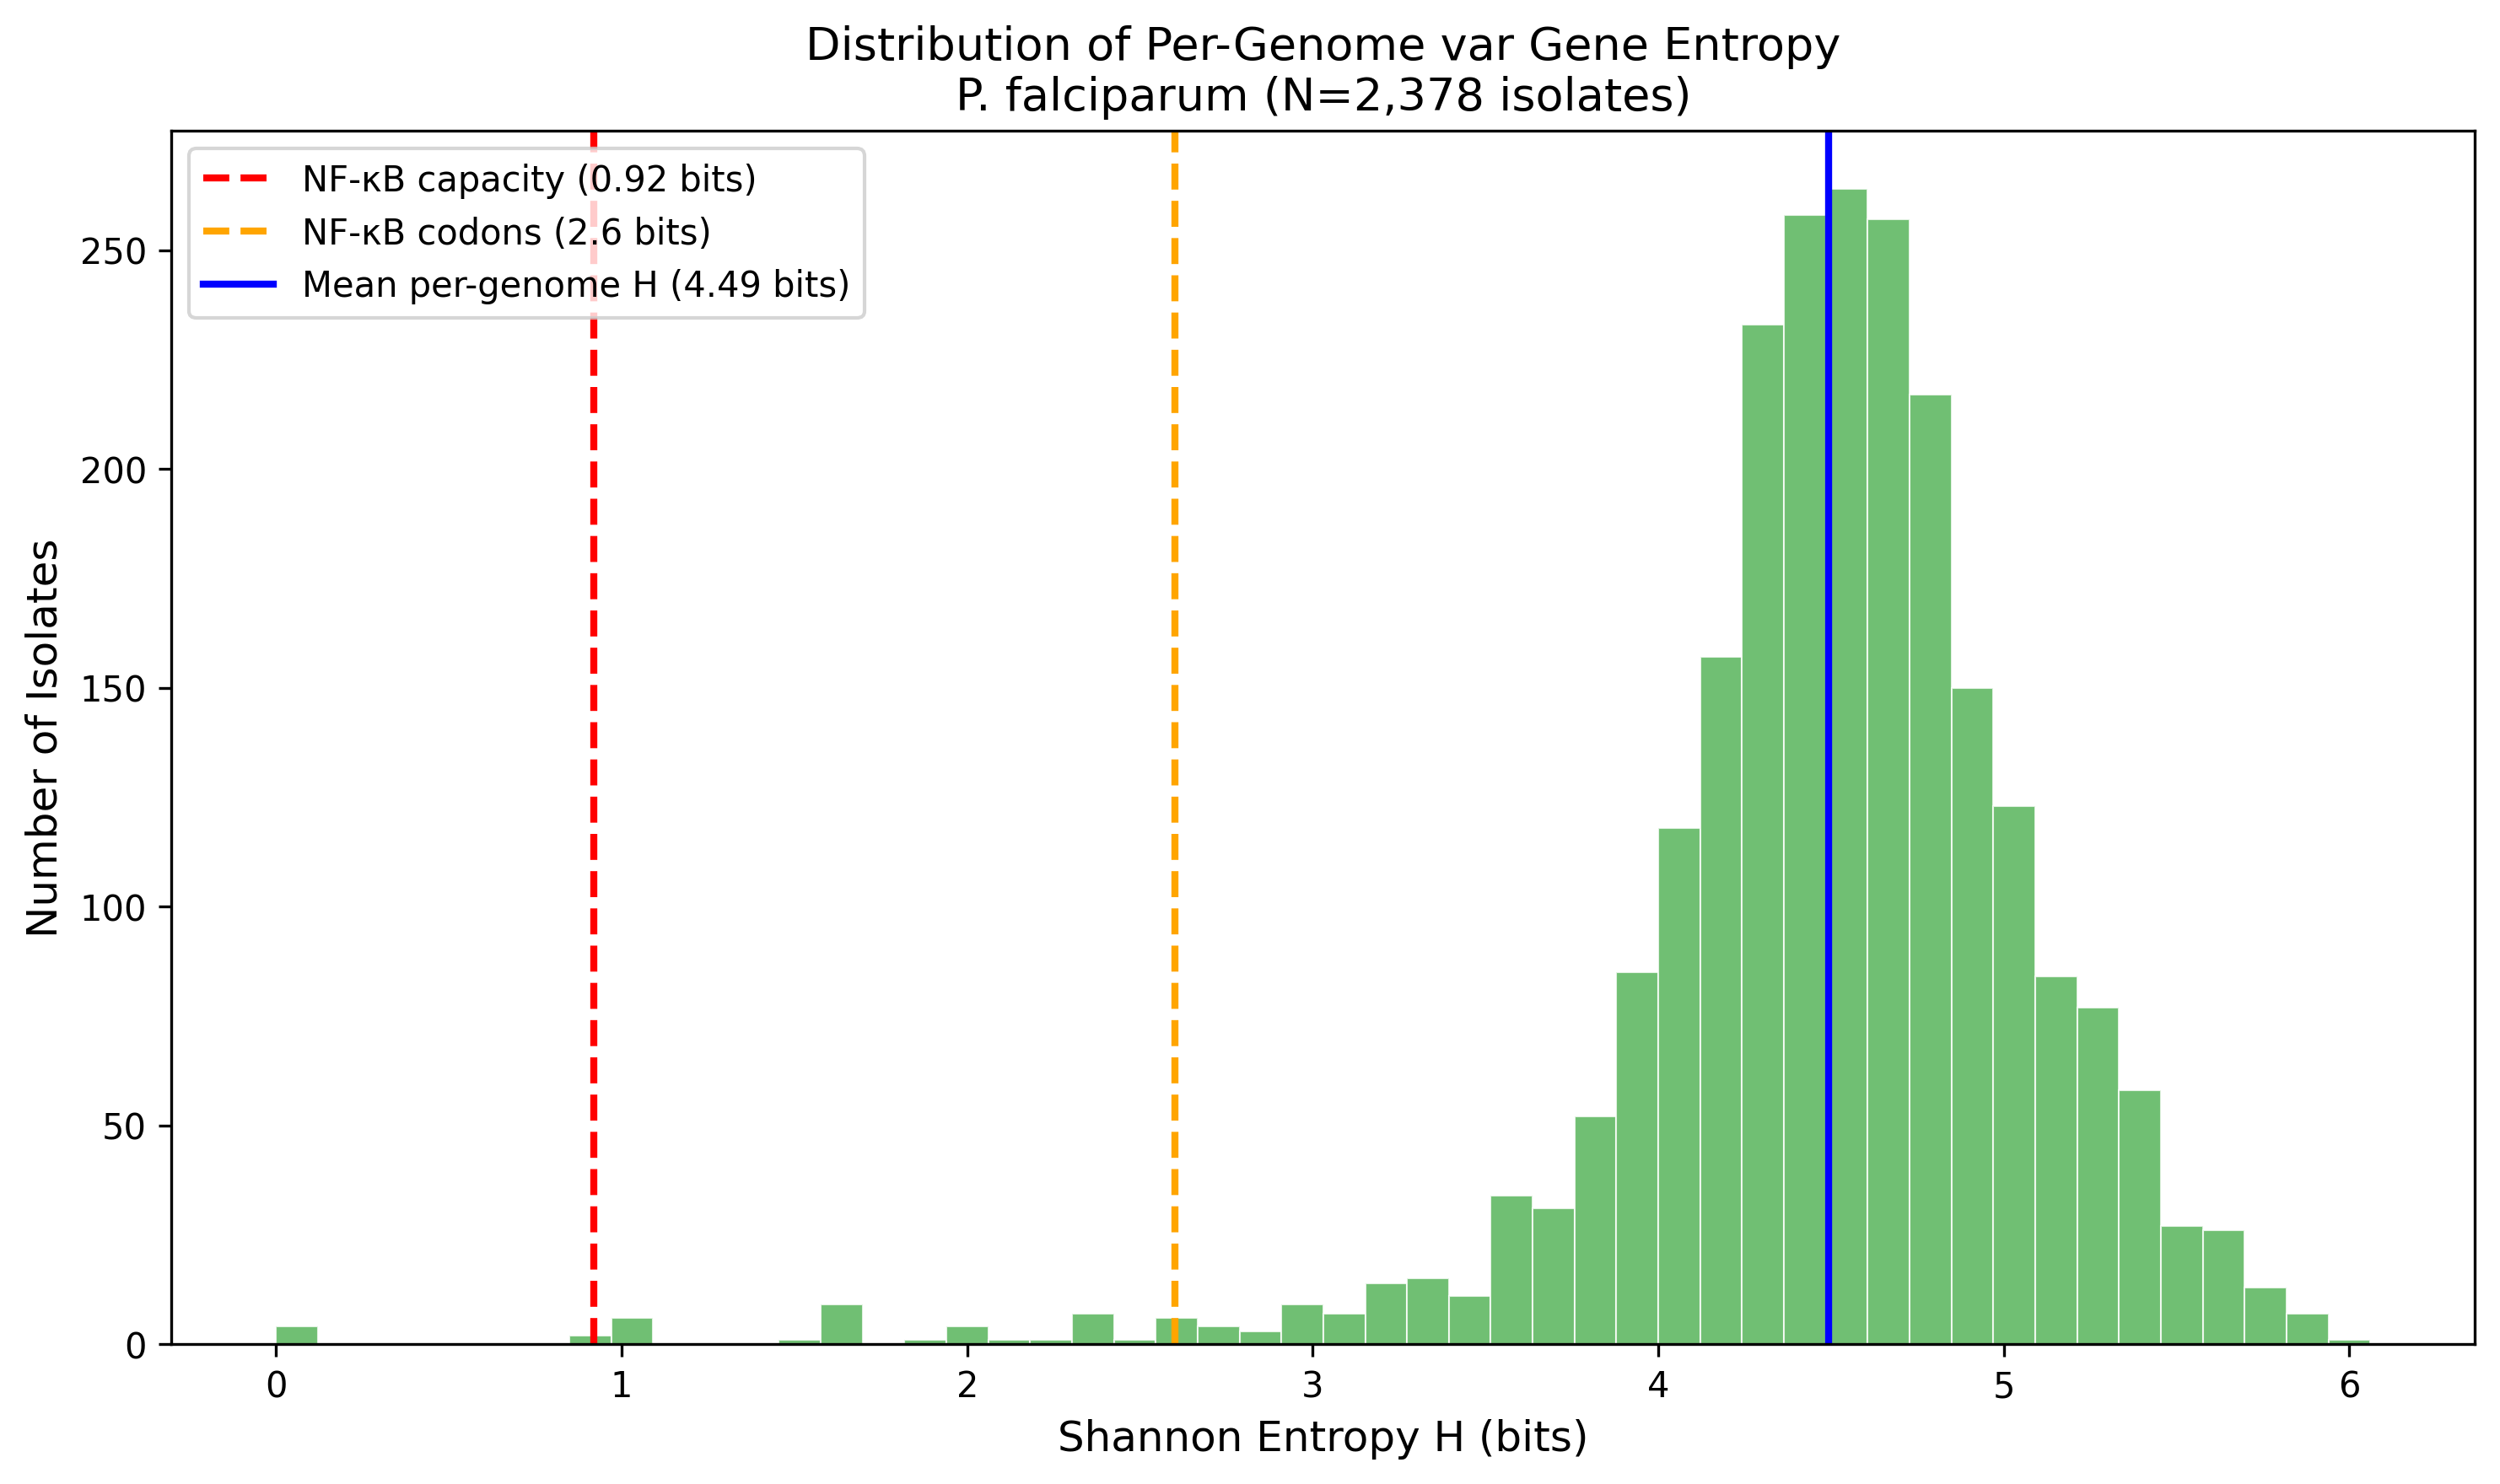
\includegraphics[width=\columnwidth]{figures/fig2_pfalciparum_per_genome_entropy.png}
\caption{Distribution of per-genome antigenic entropy across 2,378 \textit{P.~falciparum} isolates.  Mean $H = 4.49$~bits (blue line) exceeds both the NF-$\kappa$B snapshot capacity (0.92~bits, red) and signaling codon capacity (2.6~bits, orange).  This measures the sequential switching repertoire per genome, not simultaneous presentation.}
\label{fig:pergenome}
\end{figure}

\subsection{HIV-1: Extreme Diversity, Weakest Biological Match}
\label{sec:hiv}

The mean per-position Shannon entropy of the HIV-1 env protein across 496 sequences and 807 analyzable positions is:
\begin{equation}
H(X_{\text{position}}) = 2.98 \text{~bits} \quad [2.94, 3.03]
\end{equation}
This is $3.2\times$ the NF-$\kappa$B capacity and 69\% of the theoretical maximum ($\log_2 20 = 4.32$~bits per position for 20 amino acids).

The positional entropy profile reveals biologically meaningful structure: positions 1--100 (signal peptide, conserved gp120 core) show lower entropy (1.5--2.5~bits), followed by a sharp increase at positions 100--200 (variable loops V1-V2, peak at 3.81~bits), sustained high entropy through positions 200--800 (gp120 outer domain, V3-V5 loops, gp41).

\textbf{$k$-mer epitope entropy} (at MHC-I-relevant 9-mer length) is 13.94~bits over 81,566 unique 9-mers---$15.1\times$ the NF-$\kappa$B capacity.\footnote{Bootstrap CIs are not reported for 9-mer entropy because the high cardinality (81,566 types, large singleton fraction) causes systematic downward bias in resampled estimates.  The per-position CIs ($K = 20$ amino acids) are well-behaved.}

\begin{figure}[t]
\centering
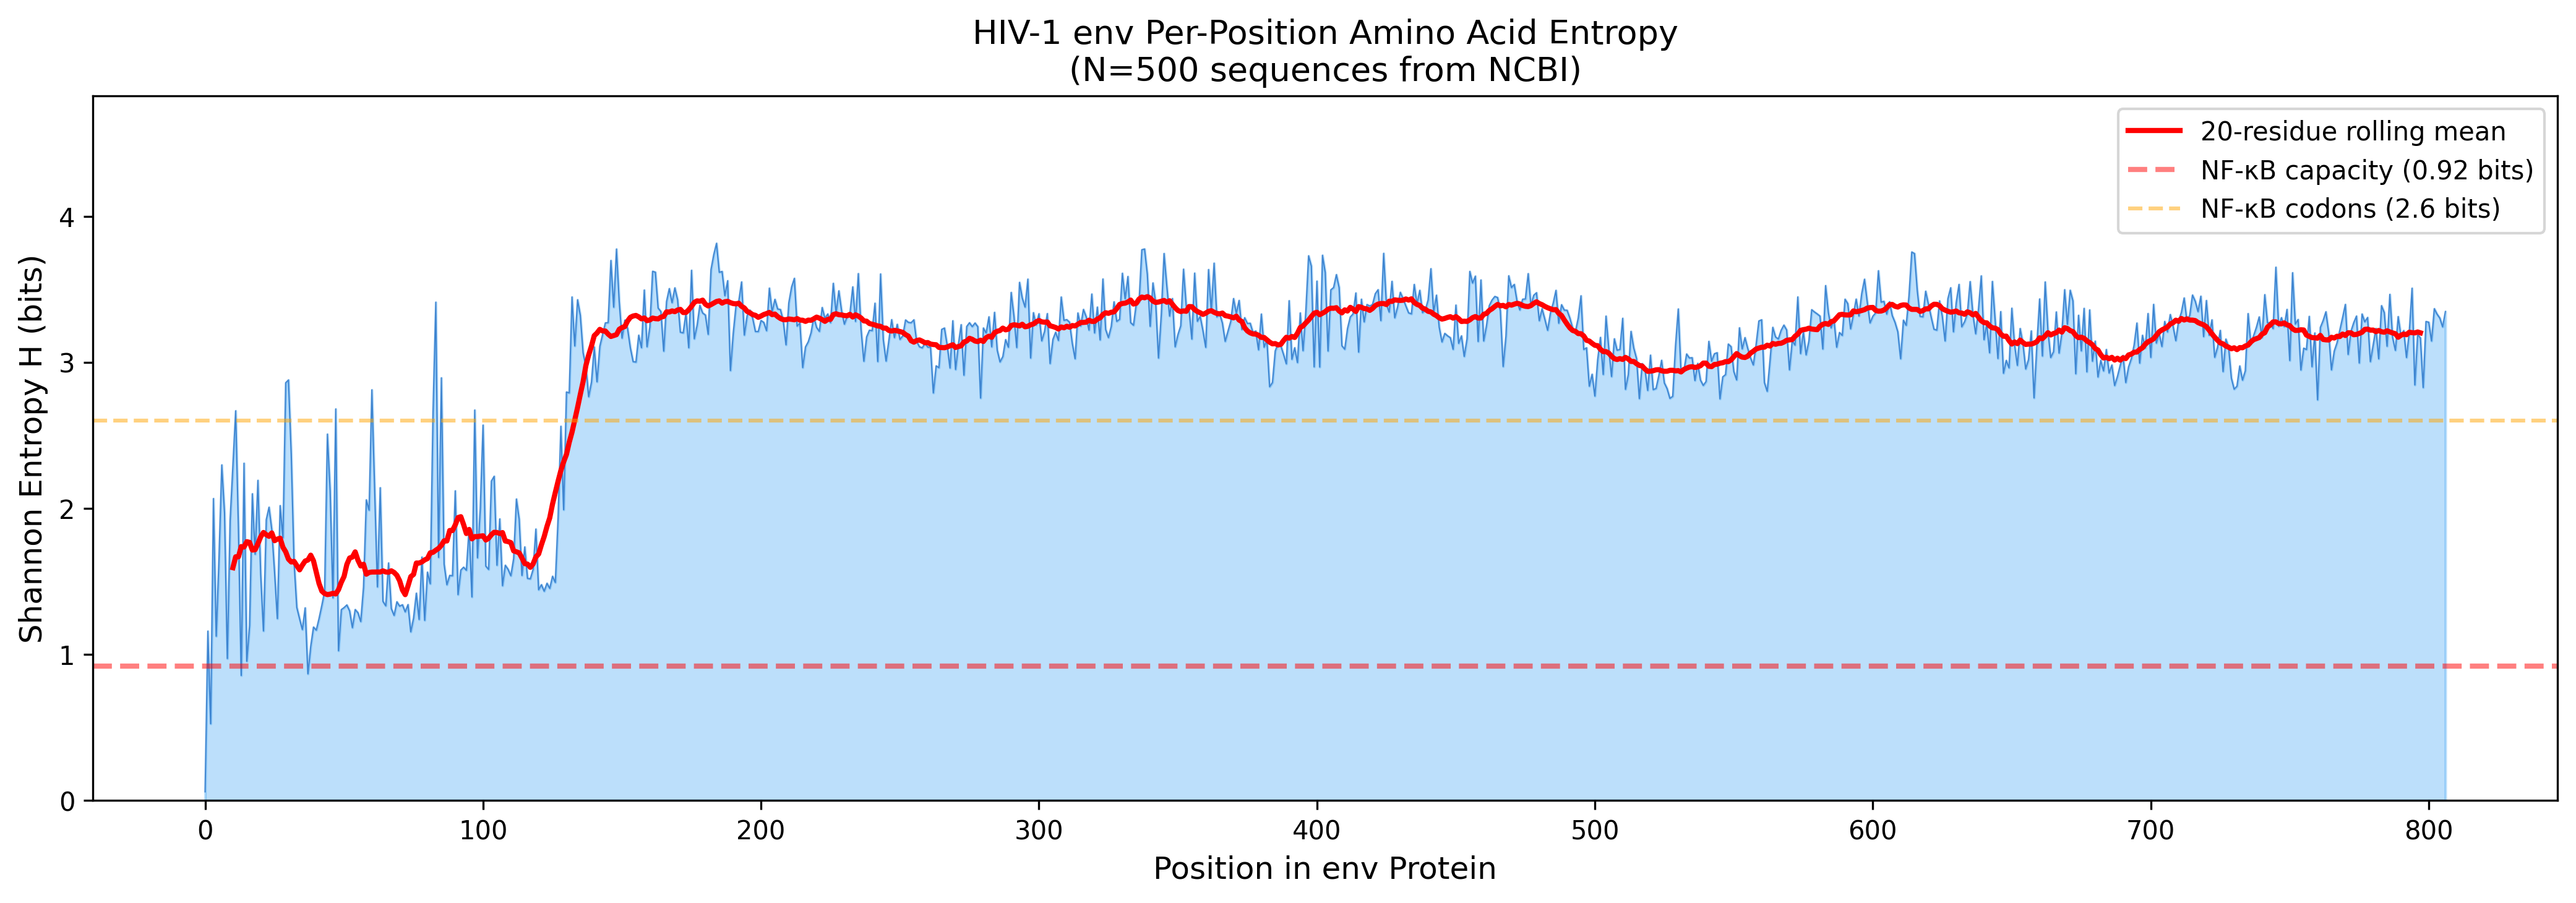
\includegraphics[width=\columnwidth]{figures/fig7_hiv_positional_entropy.png}
\caption{Per-position Shannon entropy along the HIV-1 envelope protein ($N = 496$ sequences).  Positions 100--200 (variable loops V1-V2) show peak entropy.  99.5\% of positions exceed the 0.92-bit NF-$\kappa$B capacity (lower dashed line); 85\% exceed the 2.6-bit signaling codon capacity (upper dashed line).  Red line: 20-residue rolling mean.}
\label{fig:hiv}
\end{figure}

\textbf{Caveats.}  The HIV analysis has the weakest biological match to our channel model for three reasons.  First, the 80.1\% mean pairwise divergence confirms the dataset spans multiple HIV-1 subtypes, inflating entropy relative to within-subtype diversity.  Published LANL subtype-B analyses report 1.5--2.0~bits at variable loops---still above the 0.92-bit benchmark but substantially lower than our cross-subtype estimates.  Second, our per-position entropy lacks confidence intervals at the 9-mer level due to the high cardinality problem noted above.  Third, no individual host encounters the full cross-subtype diversity; the global entropy is epidemiologically relevant but does not represent the antigenic challenge faced by a single immune system during a single infection.  Even a 50\% reduction in mean per-position entropy would yield ${\sim}1.49$~bits, still exceeding the 0.92-bit benchmark, but the margin is not as dramatic as the headline numbers suggest.

We include HIV as the most extreme data point in a spectrum, not as equally strong evidence for our framework.

\subsection{Summary Across Three Systems}

Table~\ref{tab:main} synthesizes the results.

\begin{table}[t]
\centering
\caption{Antigenic source entropy vs.\ immune channel capacity across three parasite systems.  $H/C$ ratios are computed against $C = 0.92$~bits~\citep{cheong2011}.  See text for biological caveats on each system.}
\label{tab:main}
\footnotesize
\begin{tabular}{@{}lrcr@{}}
\toprule
System & $H$ (bits) & 95\% CI & $H/C$ \\
\midrule
\textit{T.~b.} mean VSG (4 mice) & 1.70 & [1.34, 2.07] & 1.8$\times$ \\
\textit{T.~b.} max timepoint & 3.99 & --- & 4.3$\times$ \\
\textit{P.~f.} per-genome & 4.49 & [4.47, 4.52] & 4.9$\times$ \\
\textit{P.~f.} global (3,249 types) & 6.79 & [6.76, 6.79] & 7.4$\times$ \\
HIV-1 per-position env & 2.98 & [2.94, 3.03] & 3.2$\times$ \\
HIV-1 9-mer epitope & 13.94 & ---$^\dagger$ & 15.1$\times$ \\
\bottomrule
\end{tabular}
\smallskip

\footnotesize{$^\dagger$Bootstrap CIs unreliable for 9-mer entropy (81,566 types; high singleton fraction).  Per-position CI [2.94, 3.03] is well-behaved ($K = 20$).}
\end{table}

\begin{figure}[t]
\centering
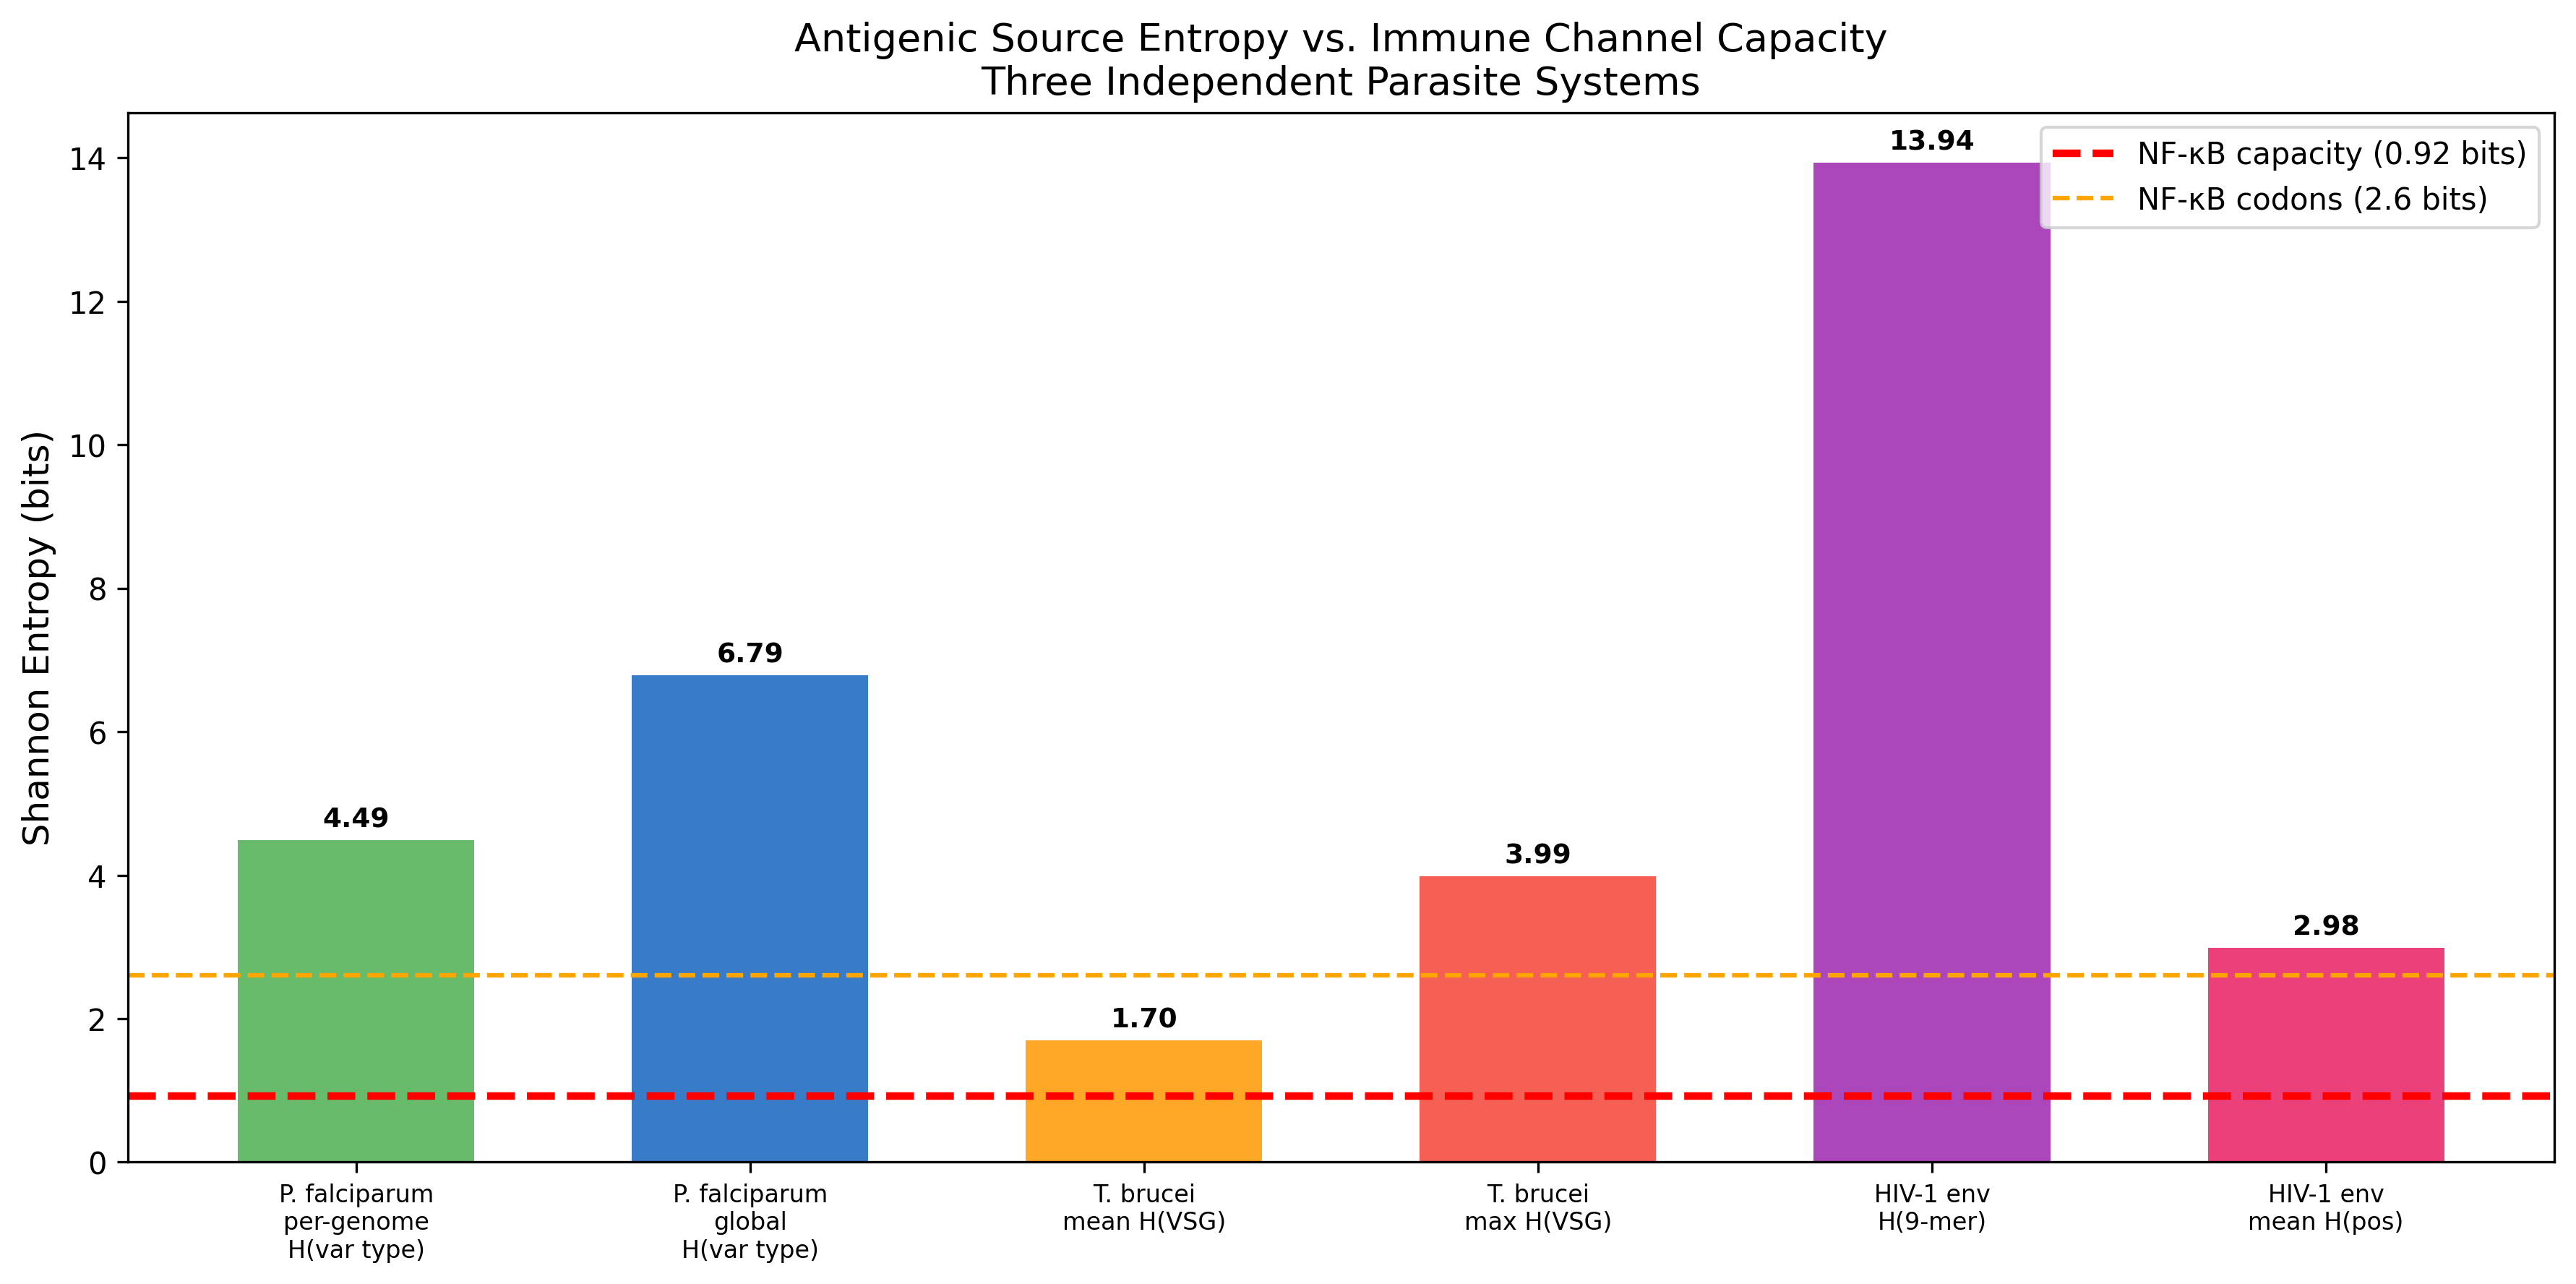
\includegraphics[width=\columnwidth]{figures/fig9_three_systems_summary.png}
\caption{Antigenic source entropy vs.\ immune channel capacity across three parasite systems.  All systems exceed the per-interaction capacity benchmark at every resolution level analyzed.  Dashed lines: published NF-$\kappa$B capacity measurements.  Strength of biological matching to the DMC model varies: strongest for \textit{T.~brucei} (temporal dynamics), intermediate for \textit{P.~falciparum} (sequential repertoire), weakest for HIV (cross-subtype inflation).}
\label{fig:summary}
\end{figure}

All three systems, at all resolution levels, produce antigenic source entropy exceeding the per-interaction signaling capacity.  The minimum ratio across all analyses is $1.6\times$ (\textit{T.~brucei} Mouse~3 mean).  Even the most conservative resolution (\textit{P.~falciparum} first-domain-only, 18 types) gives $H/C = 2.2\times$.

The key qualitative finding: antigenic entropy at measured signaling bottlenecks exceeds per-interaction capacity, and the \textit{T.~brucei} temporal dynamics are consistent with this constraint operating in vivo.  However, the immune system is a distributed adaptive network and its aggregate capacity may---indeed, almost certainly does---exceed bottleneck measurements.

\subsection{Multi-Receiver Capacity Scaling}
\label{sec:multi}

The strongest objection to our comparison: the immune system comprises ${\sim}10^{11}$ cells operating in parallel, not a single NF-$\kappa$B wire.  A single-pathway capacity of 0.92~bits understates the system's aggregate discriminative power.

The answer depends on the correlation structure among immune cells.  \citet{cheong2011} measured this directly: a population of ${\sim}14$ cells collectively achieves ${\sim}1.8$~bits---not $14 \times 0.92 = 12.9$~bits.  Capacity scales sublinearly.  Fitting both endpoints ($C(1) = 0.92$, $C(14) = 1.8$) yields:
\begin{equation}
C(M) \approx 0.92 + 0.23 \cdot \log_2(M)
\label{eq:scaling}
\end{equation}
Extrapolating: ${\sim}100$ cells yield ${\sim}2.5$~bits; ${\sim}1{,}000$ cells yield ${\sim}3.2$~bits; ${\sim}10^6$ cells yield ${\sim}5.5$~bits.

\begin{table}[t]
\centering
\caption{Multi-receiver capacity scaling: does $H > C$ survive?  $C_{\text{agg}}$ extrapolated for $10^6$ coordinated cells using Eq.~\ref{eq:scaling}.}
\label{tab:multi}
\footnotesize
\begin{tabular}{@{}lccl@{}}
\toprule
System & $H$ & $C_{\text{agg}}$ ($10^6$) & $H\!>\!C$? \\
\midrule
\textit{T.~b.} (mean) & 1.70 & ${\sim}5.5$ & No \\
\textit{T.~b.} (max) & 3.99 & ${\sim}5.5$ & No \\
\textit{P.~f.} (per-genome) & 4.49 & ${\sim}5.5$ & No \\
\textit{P.~f.} (global) & 6.79 & ${\sim}5.5$ & Yes \\
HIV-1 (per-position) & 2.98 & ${\sim}5.5$ & No \\
HIV-1 (9-mer epitope) & 13.94 & ${\sim}5.5$ & Yes \\
\bottomrule
\end{tabular}
\smallskip

\footnotesize{$H$ and $C_{\text{agg}}$ in bits.}
\end{table}

Under this scaling with $10^6$ coordinated cells, only \textit{P.~falciparum} global entropy (6.79~bits) and HIV 9-mer epitope entropy (13.94~bits) exceed the aggregate capacity of ${\sim}5.5$~bits.  The remaining measures fall below it.  The finding that $H > C$ at the per-interaction, single-pathway level is robust.  Whether it holds at the system level is an open question that depends on the correlation structure among cells---measured only for small populations (14 cells) and extrapolated here.

Three considerations temper the multi-receiver objection.  First, the logarithmic extrapolation may be optimistic: not all $10^6$ cells encounter the same antigen simultaneously, and spatial and temporal delays reduce effective coordination.  Second, the ${\sim}5.5$-bit aggregate estimate rests on a two-point extrapolation over five orders of magnitude.  Third, the \textit{T.~brucei} oscillation data provides direct empirical evidence that clearance occurs when entropy drops below ${\sim}1$~bit---consistent with a per-interaction constraint, not a ${\sim}5.5$-bit aggregate constraint, governing the effective recognition threshold.

\begin{figure}[t]
\centering
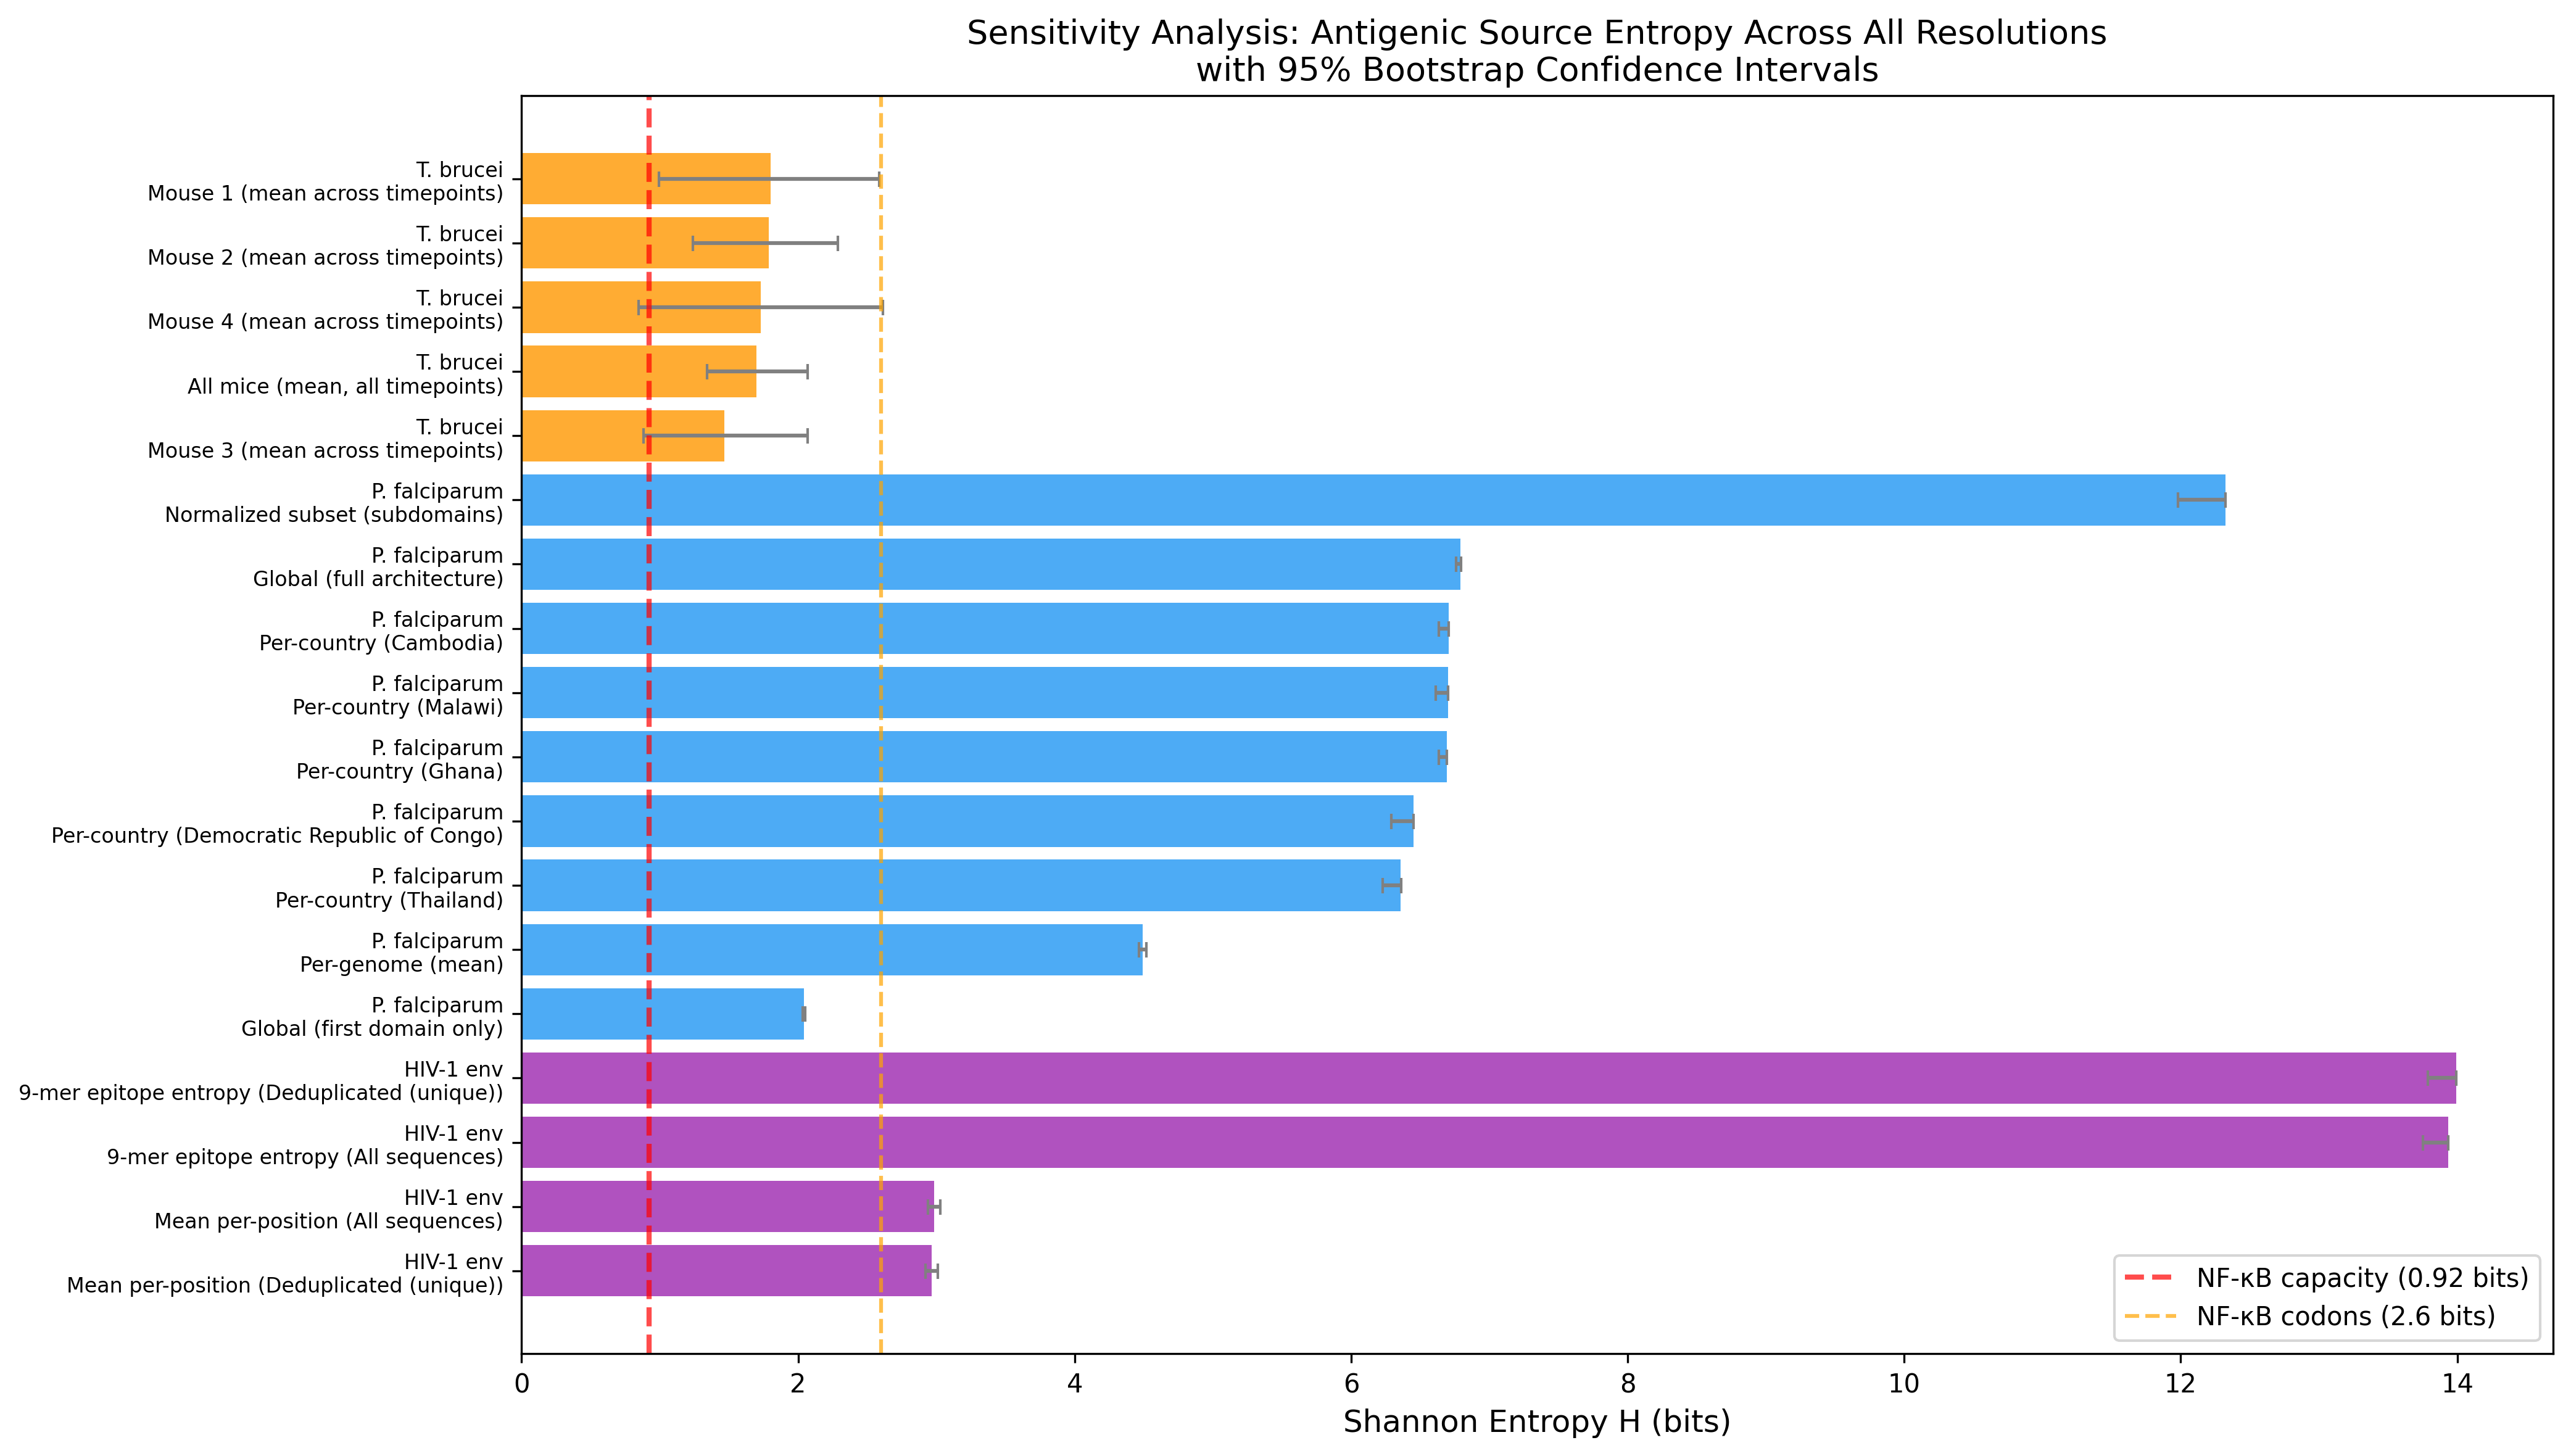
\includegraphics[width=\columnwidth]{figures/fig10_sensitivity_all_systems.png}
\caption{Sensitivity analysis: antigenic source entropy across all resolution levels with 95\% bootstrap confidence intervals.  Every measure exceeds the 0.92-bit NF-$\kappa$B capacity (red dashed line).  Blue: \textit{P.~falciparum}; orange: \textit{T.~brucei}; purple: HIV-1.}
\label{fig:sensitivity}
\end{figure}

% ============================================================
% 6. DISCUSSION
% ============================================================
\section{Discussion}
\label{sec:discussion}

\subsection{Why Does the Naive Model Work?}
\label{sec:bottleneck}

The most surprising feature of our results is that the simplest possible model---comparing repertoire entropy to single-pathway capacity---produces biologically sensible predictions.  The \textit{T.~brucei} oscillation tracks the ${\sim}1$-bit boundary, not the ${\sim}5.5$-bit aggregate estimate.  Clearance events coincide with entropy dropping below the per-interaction threshold, not below some higher system-level capacity.

We propose a \textbf{bottleneck hypothesis}: even in a massively parallel system, the aggregate performance is constrained by the per-interaction capacity at the point where individual cells make irreversible decisions.  A T~cell deciding to activate, a B~cell deciding to undergo class switching, a dendritic cell deciding which peptides to present---each of these is a single-channel-use decision that processes ${\sim}1$~bit of antigen information.  The immune system's parallelism helps by allowing \emph{many} such decisions to be made simultaneously, but each individual decision remains capacity-limited.

Consider an analogy: a room full of people each listening through a noisy telephone.  Each phone transmits 1~bit.  Having 1,000 phones does not make any single phone transmit more information---it means 1,000 independent, low-resolution decisions are made in parallel.  If the signal space contains $2^{10}$ possible messages, no individual listener can decode reliably, regardless of how many listeners there are, unless they can coordinate their observations.  The degree to which immune cells coordinate---through cytokine signaling, antigen presentation cascades, germinal center selection---determines whether the system behaves more like independent listeners (capacity stays near 1~bit per decision) or like a coordinated array (capacity scales with $M$).

The \textit{T.~brucei} data suggest that for the relevant dynamics---clearance of a dominant VSG variant---the effective constraint is closer to the single-interaction bottleneck than to the aggregate capacity.  This makes biological sense: the initial recognition event that triggers an immune response against a particular variant must pass through a signaling cascade with ${\sim}1$-bit capacity, even if the subsequent amplification and coordination involve millions of cells.

This hypothesis is testable.  It predicts that:
\begin{enumerate}
\item Clearance thresholds should correlate with single-cell signaling capacity, not with the number of responding cells.
\item Increasing the signaling capacity of individual cells (e.g., through engineered multi-feature detection) should lower the entropy threshold at which clearance occurs.
\item Parasites that reduce per-cell signaling capacity (e.g., through NF-$\kappa$B subversion, as documented by \citealt{rahman2011}) should shift the clearance threshold downward, allowing lower-entropy populations to persist.
\end{enumerate}

\subsection{Toward a Better Model}
\label{sec:better}

The DMC model served as a useful starting point because it connects to existing measurements.  But the immune system demands a richer framework.  We outline four directions, each with existing mathematical foundations that could be applied to host--pathogen data:

\textbf{Distributed adaptive inference.}  The immune system is closer to a distributed sensor network than to a single channel.  In sensor network information theory~\citep{cover2006}, the relevant quantity is the joint mutual information $I(X; Y_1, Y_2, \ldots, Y_M)$, which can exceed any individual $I(X; Y_i)$ but is bounded by the total correlation among sensors.  Measuring the joint information would require simultaneously recording antigen identity and signaling responses across multiple cells---difficult but feasible with modern single-cell techniques.

\textbf{Partially observable Markov decision processes (POMDPs).}  The immune system does not observe the full infection state; it makes decisions under partial observability based on stochastic antigen sampling.  The POMDP framework naturally captures this: the hidden state is the pathogen population composition, the observations are sampled antigens, and the actions are immune responses.  The information-theoretic constraint in a POMDP is on the observation channel, not on the decision process---aligning with our bottleneck hypothesis.

\textbf{Rate-distortion theory.}  Rather than asking whether the immune system can perfectly discriminate all variants (Shannon's zero-error criterion), rate-distortion theory asks how much discrimination error the system tolerates at a given information rate.  The immune system tolerates substantial error: not every pathogen is cleared, and not every self-antigen is tolerated.  Rate-distortion analysis would characterize the optimal tradeoff between recognition accuracy and the information cost of discrimination---a more biologically appropriate question than the zero-error capacity comparison.

\textbf{Active inference and directed information.}  The immune system does not passively observe antigens; it actively shapes the antigenic environment through clearance, inflammation, and tissue remodeling.  \citet{massey1990} introduced directed information $I(X^n \to Y^n)$ to quantify information flow in systems with feedback.  For channels with feedback, \citet{shannon1956} showed that feedback does not increase the capacity of memoryless channels, but for channels with memory---which the immune system certainly is---feedback \emph{can} increase capacity~\citep{coverpombra1989}.  Computing directed information from paired temporal data of antigenic variation and immune response would quantify this feedback benefit.

Each of these frameworks addresses specific limitations of the DMC model.  None has been applied to host--pathogen data.  We propose them as the natural next steps, not as corrections that invalidate our current findings---the bottleneck comparison remains informative even as the full-system model awaits development.

\subsection{Convergent Evolution and Theoretical Context}
\label{sec:convergence}

Three phylogenetically unrelated lineages---\textit{Plasmodium} (Apicomplexa), \textit{Trypanosoma} (Kinetoplastida), and HIV (Retroviridae)---independently evolved antigenic repertoires whose entropy exceeds per-interaction signaling capacity.  This convergence is consistent with strong selection pressure toward the $H > C$ regime at the bottleneck level.

The theoretical context for this convergence comes from two frameworks, which we treat as inspiration rather than formal models of the biological system.

The arbitrarily varying channel (AVC)~\citep{blackwell1960,csiszar1988} provides a game-theoretic lens.  An AVC is defined by a family $\{W(y|x,s) : s \in \mathcal{S}\}$, where an adversary chooses a state $s$ to maximize decoding error.  The Csisz\'{a}r-Narayan dichotomy theorem establishes that an adversary can drive deterministic-code capacity to zero if it achieves ``symmetrizability''---the ability to perfectly mimic legitimate signals.  No biological parasite achieves this; molecular mimicry is always imperfect, and pathogen-associated molecular patterns provide side information that cannot be disguised without loss of function.  But the AVC framework establishes the \emph{direction} of selection pressure: strategies that increase antigenic entropy relative to channel capacity move toward the symmetrizability horizon.

Evolutionary game theory provides the selection argument.  \citet{bergstrom2005} proved that the fitness value of environmental information equals the mutual information between cue and environment.  A parasite that reduces the mutual information between its antigens and the immune response---by increasing antigenic entropy beyond channel capacity---directly reduces the fitness value of the immune system's information channel.

However, many parasites adopt strategies other than antigenic variation---intracellular hiding, rapid transmission before clearance, direct immunosuppression---that do not require large antigenic repertoires.  The claim is narrower than ``all parasites must evolve $H > C$'': antigenic variation, \emph{when it evolves}, faces selection pressure toward entropy levels that exceed per-interaction signaling capacity.  The three lineages we study are the canonical examples of this strategy, and all three exceed the bottleneck benchmark.

\subsection{Limitations}

\textbf{Channel capacity comparison is indirect.}  We compare parasitic source entropy to published immune channel capacity measurements made in different experimental systems (mouse macrophages for NF-$\kappa$B, \emph{in vivo} human and murine infections for antigenic variation).  The definitive test---measuring channel capacity in immune cells \emph{during} parasitic infection---has not been performed.

\textbf{Shannon entropy overstates effective diversity.}  Not all var genes or VSGs are equally immunogenic.  Functional constraints reduce the effective antigenic space below sequence-level diversity.  Shannon entropy treats every distinct sequence as an equally informative symbol.  Our entropy estimates are therefore upper bounds on the immunologically relevant diversity.

Three features mitigate this concern.  First, we compute entropy over \emph{domain architectures} rather than raw sequences for \textit{P.~falciparum}---a functionally relevant classification.  Second, our sensitivity analysis spans three orders of magnitude in classification granularity, and the $H > C$ finding holds at every level.  Third, for HIV, the concentration of entropy at immune-facing surfaces (variable loops: ${\sim}3.0\text{--}3.8$~bits) versus buried residues (conserved core: ${\sim}1.5\text{--}2.5$~bits) is consistent with immunologically targeted diversity.

\textbf{HIV cross-subtype inflation.}  Our HIV dataset spans multiple subtypes, inflating per-position entropy.  Single-subtype analysis would give lower but likely still capacity-exceeding values (published LANL subtype-B analyses report 1.5--2.0~bits at variable loops).

\textbf{\textit{P.~falciparum} sequential expression.}  Only one var gene is expressed at a time.  Global entropy measures the repertoire, not the instantaneous challenge.  Per-genome entropy of 4.49~bits should be interpreted as the upper bound on cumulative antigenic burden across chronic infection.

\textbf{The DMC model is approximate.}  The immune system has memory, feedback, and non-stationarity---all of which violate DMC assumptions.  We have addressed this limitation explicitly in Section~\ref{sec:dmc} and proposed richer frameworks in Section~\ref{sec:better}.  The DMC comparison remains informative as a bottleneck analysis, but the full-system implications require more sophisticated models.

\textbf{Two-point extrapolation for multi-receiver scaling.}  Our $C(M) \approx 0.92 + 0.23 \cdot \log_2(M)$ scaling law rests on just two data points ($M = 1$ and $M = 14$).  The true scaling for $M = 10^6$ could be substantially different.

% ============================================================
% 7. CONCLUSION
% ============================================================
\section{Conclusion}
\label{sec:conclusion}

We measured antigenic entropy exceeding per-interaction signaling capacity in three systems.  The results, ordered by strength of evidence:

\begin{enumerate}
\item \textbf{\textit{T.~brucei}: strongest evidence.}  VSG entropy oscillates between 0.04 and 3.99~bits, crossing the ${\sim}1$-bit capacity threshold repeatedly during infection.  The rate of antigenic novelty (${\sim}0.04\text{--}0.06$~bits/day) approximately matches the rate of immune learning (${\sim}0.07\text{--}0.14$~bits/day), consistent with the observed chronic-but-survivable infection dynamics.  This is the most direct empirical observation of a biological system whose temporal dynamics track a Shannon capacity boundary.

\item \textbf{\textit{P.~falciparum}: supporting evidence with caveats.}  Per-genome repertoire entropy of 4.49~bits exceeds per-interaction capacity by $4.9\times$, but only one variant is expressed at a time.  The entropy measures the sequential switching repertoire, not simultaneous load.

\item \textbf{HIV-1: extreme case, weakest match.}  Per-position entropy of 2.98~bits and 9-mer entropy of 13.94~bits produce the largest $H/C$ ratios, but cross-subtype inflation and the lack of per-position confidence intervals at the $k$-mer level weaken the comparison.
\end{enumerate}

The immune system is not a single NF-$\kappa$B wire, and we do not claim that the $H > C$ inequality at the per-interaction level implies system-level failure of immune recognition.  What we do claim is that individual immune cells make decisions at ${\sim}1$~bit of antigenic information per signaling event, that three unrelated parasite lineages independently evolved repertoire entropies exceeding this bottleneck, and that the \textit{T.~brucei} temporal dynamics are consistent with this bottleneck operating as a meaningful constraint on infection dynamics.

The bottleneck hypothesis---that aggregate immune performance is constrained by per-interaction signaling capacity at the point of individual cell decision---is testable.  It predicts that clearance thresholds correlate with single-cell capacity, that engineered capacity enhancement would shift clearance thresholds, and that parasitic subversion of signaling pathways would degrade clearance.

The decisive next steps are: (1)~measure immune signaling capacity \emph{during} infection, replicating the \citet{cheong2011} protocol in \textit{Toxoplasma}-infected macrophages or \textit{Plasmodium}-exposed immune cells; (2)~compute mutual information $I(\text{antigen}; \text{response})$ from paired longitudinal data of antigenic variation and immune response, which would measure actual channel throughput under parasitic attack rather than comparing independently measured source entropy and capacity benchmarks.

% ============================================================
% DATA AND CODE AVAILABILITY
% ============================================================
\section*{Data and Code Availability}

Analysis code and processed data are available at \url{https://github.com/novalis78/Parasitology-Information-Theory}.  \textit{T.~brucei} VSG-seq data from \citet{mugnier2015} via supplementary databases and GitHub (github.com/mugnierlab).  \textit{P.~falciparum} var gene data from \citet{otto2019} via Zenodo (doi:10.5281/zenodo.3549732).  HIV-1 env sequences from NCBI Protein Database.

% ============================================================
% ACKNOWLEDGMENTS
% ============================================================
\section*{Acknowledgments}

The authors thank the Mugnier laboratory for making VSG-seq data publicly available, the developers of the varDB database (Thomas Otto and colleagues), and the NCBI for programmatic access to HIV sequence data.

% ============================================================
% REFERENCES
% ============================================================
{\small
\setlength{\bibsep}{2pt plus 0.5pt minus 0.5pt}
\bibliography{references}
}

\end{document}
